\scanpage{48}
I want to characterize $A$ in terms of $\widehat\Sigma^*, A^*\in\widehat\Sigma^*$ (in the case $A\in\Sigma$). Of course, $A$ is a \deleted{\unsure{segment|segment}} segment which contains $A^*$, and as $A^*\supset\partial A$, it is minimal (\deleted{\unsure{the only one|the one}} that works) among the segments \inserted{of $S$} which contain\deleted{\unsure{s}} $A^*$ -- but this is not enough to characterize it. It has however the additional property,
\[
 \forall B^*\in\widehat\Sigma^*,\quad\text{\unsure{we have}}\quad B^*\cap A=\phi,\quad\text{or }B^*\subset A
\]

\uline{NB} In fact, with only the conditions $\sigma1:\sigma3$ on $\Sigma$, \deleted{\unsure{it|in|i}} it is not true that knowledge of $\widehat\Sigma^*$ gives back $\Sigma$, example

\figure{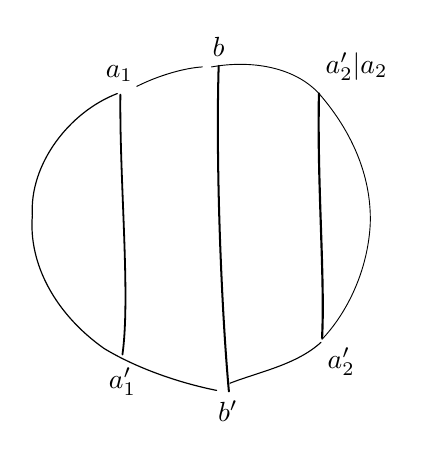
\begin{tikzpicture}[x=.013cm,y=-.013cm,line cap=round,line join=round]
\draw[line width=.43pt] (232,1287) .. controls (185,1305) and (146,1356) .. (149,1406) .. controls (145,1453) and (171,1502) .. (219,1536) .. controls (252,1556) and (294,1570) .. (329,1577);
\draw[line width=.35pt] (251,1280) .. controls (273,1269) and (298,1262) .. (315,1261);
\draw[line width=.33pt] (324,1261) .. controls (363,1254) and (405,1261) .. (429,1287) .. controls (463,1326) and (481,1371) .. (479,1416) .. controls (476,1464) and (454,1504) .. (432,1527);
\draw[line width=.40pt] (431,1530) .. controls (407,1552) and (370,1559) .. (342,1570);
\draw[line width=.65pt] (235,1288) .. controls (234,1372) and (245,1485) .. (237,1542);
\draw[line width=.73pt] (331,1260) .. controls (328,1360) and (334,1502) .. (341,1578);
\draw[line width=.78pt] (429,1287) .. controls (427,1374) and (435,1468) .. (432,1526);
\node[above] at (234,1285) {$a_1$};
\node[above] at (331,1260) {$b$};
\node[above right] at (426,1284) {$\unsure{a'_2|a_2}$};
\node[below] at (237,1545) {$a'_1$};
\node[below] at (340,1578) {$b'$};
\node[below right] at (428,1526) {$a'_2$};
\end{tikzpicture}}
equivalence relation \inserted{$\mathcal R$} with three classes $\{a_1,a'_1\}$ $\{b,b'\}$ $\{a_2,a'_2\}$, \inserted{\unsure{define here|let us define}} $\Sigma_1$ formed of the segments $\{a_i,a'_i\}$ \deleted{$\{a,a'\}$} $(i\in\{1,2\})$, and $\{a_1,a'_1,b,b'\}$ and $\Sigma_2$ defined symmetrically, define the same $\mathcal R$\unsure{.|*}

\deleted{More general \unsure{example|statement}: one \unsure{can} in a \unsure{unique} way \unsure{give} $\Sigma$ so as to give}
\[
 \begin{aligned}
 &\left\{\begin{aligned}
   &\deleted{\widehat\Sigma^*=\mathcal R,\quad\text{\uuline{and}}}\\
   &\deleted{\dot R\overset{\text{definition}}{=}S\setminus\coprod_{A\in\Sigma} A=\unsure{S'|S_1|S_i},}
 \end{aligned}\right.\\
 &\qquad\deleted{\text{\unsure{element|element} \uline{given} in}}\\
 &\qquad\deleted{\text{advance of }\mathcal R}\\
 &\qquad S'\ \text{not a segment}
 \end{aligned}
\]
% archive sheet number: 47
